\chapter{Graph Tracking in Probabilistic Models}
\label{cha:graph-track-prob}

We will now see how the system described in chapter~\ref{cha:impl-dynam-graph}, implemented in the
Julia package \irtrackerjl{}, can be utilized for the analysis of probabilistic models written in
\dppljl{}, and for posterior inference in \turingjl{}.  This part of the work is realized in another
package, \autogibbsjl{}, which is also available as open-source
code\footnote{\url{https://github.com/phipsgabler/AutoGibbs.jl}}.  There are two applications
provided, built on top of the graph tracking functionality: first, dependency analysis of random
variables in a model.  The result is a complete graphical model for static models, and a slice of it
for dynamic models.  This graph can be plotted for visualization.  Second, given the dependency
graph, the conditional likelihoods of unobserved variables in static models can be extracted.  With
these, analytic Gibbs conditionals for certain variables can be derived and used in \turingjl{}'s
within-Gibbs sampler.

\section{Dependency Analysis in Dynamic Models}
\label{sec:dependency-analysis}

In order to apply \irtrackerjl{} to extract the dependencies in a probabilistic model written in
\dppljl{}, recall the internal structure of such models.  As was introduced in
section~\ref{sec:prob-prog}, there is one evaluator function, into which the original code is
transformed, and which evaluates the model in different modes.  This function has the same structure
as the original code, but adds some more complicated book-keeping logic to it, and transforms the
tilde statements into function calls with additional metadata.  Furthermore, when using the model as
a callable object, there are several layers of dispatch (about five layers of nesting, depending on
the arguments), until the real evaluator function is actually hit.  There is no further nesting
involved beyond the evaluator function, though (\turingjl{} currently does not support nested
models).

Therefore, we first need to introduce an \irtrackerjl{} context that will record all the internal
function calls down to the evaluator function, and stop there.  Similar to the
\jlinl{DepthLimitContext} demonstrated on page~\pageref{lst:depthlimitcontext}, the main task here
is to overload the \jlinl{canrecur} method to stop at the right call.  This can easily be done by
introducing a helper predicate function \jlinl{ismodelcall} that dispatches on the involved types.
Next, we notice that the resulting computation graph consists of a nested and quite complicated
structure, due to the initial levels of nesting.  To work with the core model structure, we need to
remove outer layers from the innermost node containing the trace of the evaluator function.
Finally, many of the statements in the trace of the evaluator function do not have relevance for
dependency analysis~-- like those that stem from internal calculations done by the model, or
statements that were written by the user but to not lie on the dependency graph, such as debugging
statements or parts of loops.  These can be stripped off in advance, so as to clean the raw
dependency trace.  The three preparation steps are put together in one method:
\begin{lstlisting}
function slicedependencies(model::Model{F}, args...) where {F}
    trace = trackmodel(model, args...)
    strip = strip_model_layers(F, trace)
    slice = strip_dependencies(strip)
    return slice
end
\end{lstlisting}
where \jlinl{trackmodel} extracts the computation graph with the context for models tracking,
\jlinl{strip_model_layers} removes the outer method calls, and \jlinl{strip_dependencies} removes
all SSA code that is not on the dependency graph spanned by the sampling statements.

The final and most intricate step is to add all the remaining SSA statements to a new graph
structure, describing a more domain-specific representation.  In this \jlinl{Graph} type, only
assumption, observation, call, and constant nodes remain, storing relevant metadata such as their
values, variable names, and distribution objects.  In addition, the object contains intermediate
information used during graph construction, such as the mapping between newly generated and original
references.  The graph construction is implemented in a function \jlinl{makegraph}.  The final graph
dependency tracking interface thus consists of the single function
\begin{lstlisting}
function trackdependencies(model, args...)
    slice = slicedependencies(model, args...)
    return makegraph(slice)
end
\end{lstlisting}
There are two complications regarding \jlinl{makegraph}.  For one, model arguments are handled
specially by \dppljl{}~-- there are some internal arguments added, and the original arguments are
inspected to allow, e.g., to run the same model in prior or likelihood contexts.  This part needs to
be sorted out, so that the passed argument values are correctly set up as constants in the
dependency graph.  Since all information is present, the task is resolved by correctly identifying
the arguments and restructuring their contents into the right form.

The other problem is the handling of mutation, and tracking of modified array elements.  For
example, a hidden Markov model with states \jlinl{s} and transition matrix \jlinl{T} might contain
code like this:
\begin{lstlisting}
s = zeros(Int, N)
s[1] ~ Categorical(K)
for i = 2:N
    s[i] ~ Categorical(T[s[i-1]])
end
\end{lstlisting}
In order to model the dependency between successive elements of \jlinl{s}, an empty array is first
set up, and then subsequently populated by the results of the tilde statements describing the Markov
process.  In this form, only the individual variables \jlinl{s[i]} are \enquote{seen} by the
inference algorithm.  Internally, the respective tilde statements are translated to array
assignments of the form \jlinl{s[i] = tilde_assume(...)}, but with additional lowering of the
involved arguments, after which the corresponding IR will look approximately like this:\todo{page break}
\begin{lstlisting}
%9 = %i - 1                                  # i - 1
%10 = getindex(%s, %9)                       # s[i - 1]
%11 = getindex(%T, %10)                      # T[s[i - 1]]
%12 = VarInfo{:s}(((%i,),))
%13 = Categorical(%11)
%14 = tilde_assume(..., %13, ..., %12, ...)  # %14 ~ %13
%15 = setindex!(%s, %14)                     # s[i] = %14
\end{lstlisting}
(which is not real SSA form~-- several statements have been collapsed, and letters been used in SSA
variables for clarity.)  We see that the direct association between the original variable
\jlinl{s[i]} (within \jlinl{\%s}) and its distribution (\jlinl{\%13}) is not preserved in the line
of the tilde method, but spread over multiple statements.  Even worse, since all statements for the
different \jlinl{s[i]} result in mutating \jlinl{setindex!} calls on \jlinl{\%s}, the immediate
dependency between \jlinl{s[i]} and \jlinl{s[i-1]} is not available structurally, but must be
recovered dynamically.

The \jlinl{makegraph} implementation solves this by successively identifying mutated arrays
representing random variables through inspection of the indexing calls around tilde statements, and
storing the association between the assumption and the array elements.  This part of the procedure
is the most intricate one, and there may exist cases where mutation is able to \enquote{circumvent}
the dependency analysis.  Additionally, the matching between indexing arguments involves some
careful treatment of variable names; the existing \dppljl{} API for this functionality is not very
comprehensive.  Due to this, the implementation of \autogibbsjl{} currently only supports
\enquote{simple} indexing by one tuple of integers.  Other, more general indexing styles allowed in
Julia could be added in future extensions.  Furthermore, broadcasting tilde statements, that are
supported in \dppljl{}, are not supported by \autogibbsjl{} at the moment.

\newthought{To illustrate} the extracted dependency graphs obtained by \autogibbsjl{}, we will
examine the two simple models shown in listing~\ref{lst:dependency-examples}: a Boolean variable
sampled from a mixture of two Bernoulli distributions, and a simple single-variable Gaussian model
with conjugate prior.\todo{fix caption alignment} The pretty-printed \jlinl{Graph} objects resulting
from each model are shown below them, in listing~\ref{lst:trace-examples}.  We can see that the
model arguments for observations occur as constant values, and all of the intermediate function
calls visible in the original model definitions are preserved.  From this structure, \autogibbsjl{}
can construct output in the Dot graph format and visualized using GraphViz
\parencite{gansner2000open}.  The rendered output of the example models is shown in
figure~\ref{fig:geom-deps}.\todo{orphan}

\begin{lstfloat}[p]
\begin{lstlisting}[style=lstfloat]
@model function bernoulli_mixture(x)
    w ~ Dirichlet(2, 1/2)
    π ~ DiscreteNonParametric([0.3, 0.7], w)
    x ~ Bernoulli(π)
end

@model function hierarchical_gaussian(x)
    λ ~ Gamma(2.0, inv(3.0))
    m ~ Normal(0, sqrt(1 / λ))
    x ~ Normal(m, sqrt(1 / λ))
end
\end{lstlisting}
  \caption{Two simple example models: a mixture of two Bernoulli random variables with fixed
    probabilities, and a Gaussian model with conjugate prior.  Both models are defined over one
    single observation.}
  \label{lst:dependency-examples}
\end{lstfloat}

\newsavebox{\bernoullitrace}
\begin{lrbox}{\bernoullitrace}
\begin{lstlisting}[style=lstfloat]
⟨2⟩ = false
⟨3⟩ = Dirichlet(2, 0.5) → Dirichlet{Float64}(alpha=[0.5, 0.5])
⟨4⟩ = w ~ ⟨3⟩ → [0.82, 0.17]
⟨5⟩ = DiscreteNonParametric([0.3, 0.7], ⟨4⟩) → DiscreteNonParametric{...}(
        support=[0.3, 0.7], p=[0.82, 0.17])
⟨6⟩ = π ~ ⟨5⟩ → 0.3
⟨7⟩ = Bernoulli(⟨6⟩) → Bernoulli{Float64}(p=0.3)
⟨8⟩ = x ~ ⟨7⟩ ← ⟨2⟩
\end{lstlisting}
\end{lrbox}
\newsavebox{\gaussiantrace}
\begin{lrbox}{\gaussiantrace}
\begin{lstlisting}[style=lstfloat]
⟨2⟩ = 1.4
⟨3⟩ = Gamma(2.0, 0.33) → Gamma{Float64}(α=2.0, θ=0.33)
⟨4⟩ = λ ~ ⟨3⟩ → 0.92
⟨5⟩ = /(1, ⟨4⟩) → 1.08
⟨6⟩ = sqrt(⟨5⟩) → 1.03
⟨7⟩ = Normal(0, ⟨6⟩) → Normal{Float64}(μ=0.0, σ=1.03)
⟨8⟩ = m ~ ⟨7⟩ → 1.85
⟨9⟩ = /(1, ⟨4⟩) → 1.08
⟨10⟩ = sqrt(⟨9⟩) → 1.03
⟨11⟩ = Normal(⟨8⟩, ⟨10⟩) → Normal{Float64}(μ=1.85, σ=1.03)
⟨12⟩ = x ~ ⟨11⟩ ← ⟨2⟩
\end{lstlisting}
\end{lrbox}
\begin{lstfloat}[p]
  \loosesubcaptions
  \subbottom[Trace of \texttt{bernoulli\_mixture(false)} (some type parameters not shown).\hfill]{%
    \usebox{\bernoullitrace}}
  \subbottom[Trace of \texttt{hierarchical\_gaussian(1.4)}.\hfill]{%
    \usebox{\gaussiantrace}}
  \caption{Traced structure of the two example models introduced above, with fixed observations
    \texttt{false} and \texttt{1.4}.  Values in \(\langle\)angle brackets\(\rangle\) denote
    intermediate values (similar to SSA variables), and right arrows denote the resulting values of
    function calls.  The left arrow indicates the source of the observed value.  Decimal parts have
    been truncated for better readability.}
  \label{lst:trace-examples}
\end{lstfloat}

\FloatBlock

\begin{figure}[p]
  \centering
  \subbottom[][\texttt{bernoulli\_mixture(false)}]{%
    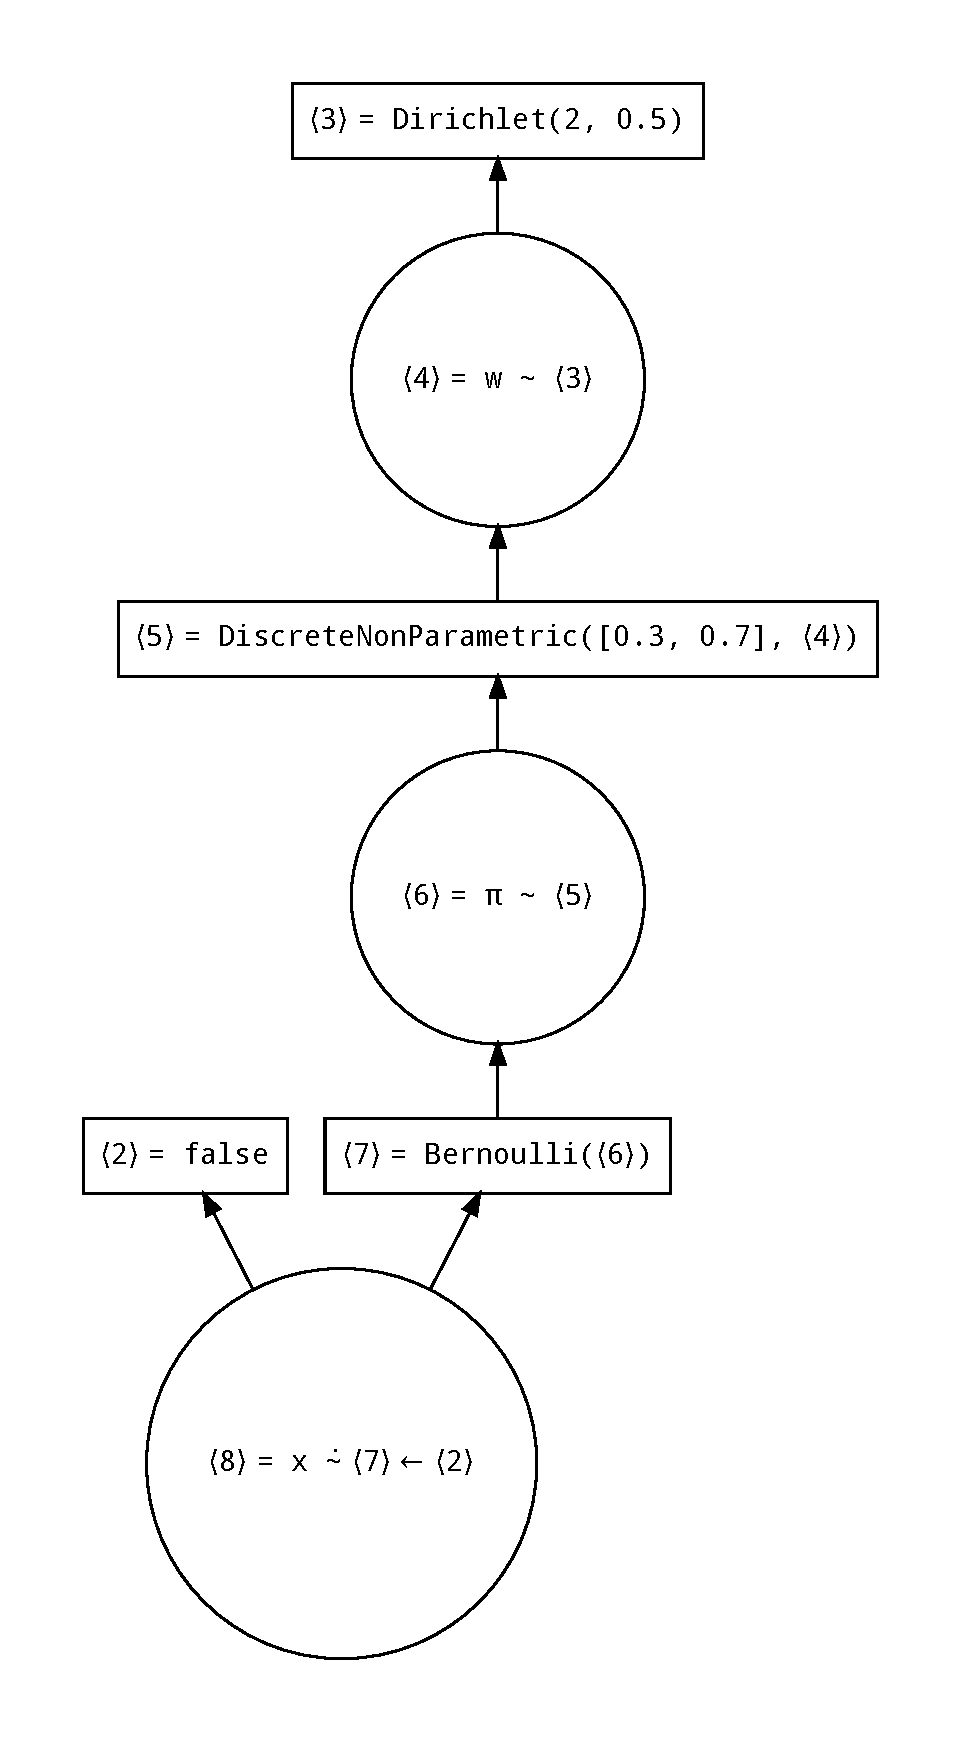
\includegraphics[width=0.49\textwidth]{figures/bernoulli_dependencies}}
  \subbottom[][\texttt{hierarchical\_gaussian(1.4)}]{%
    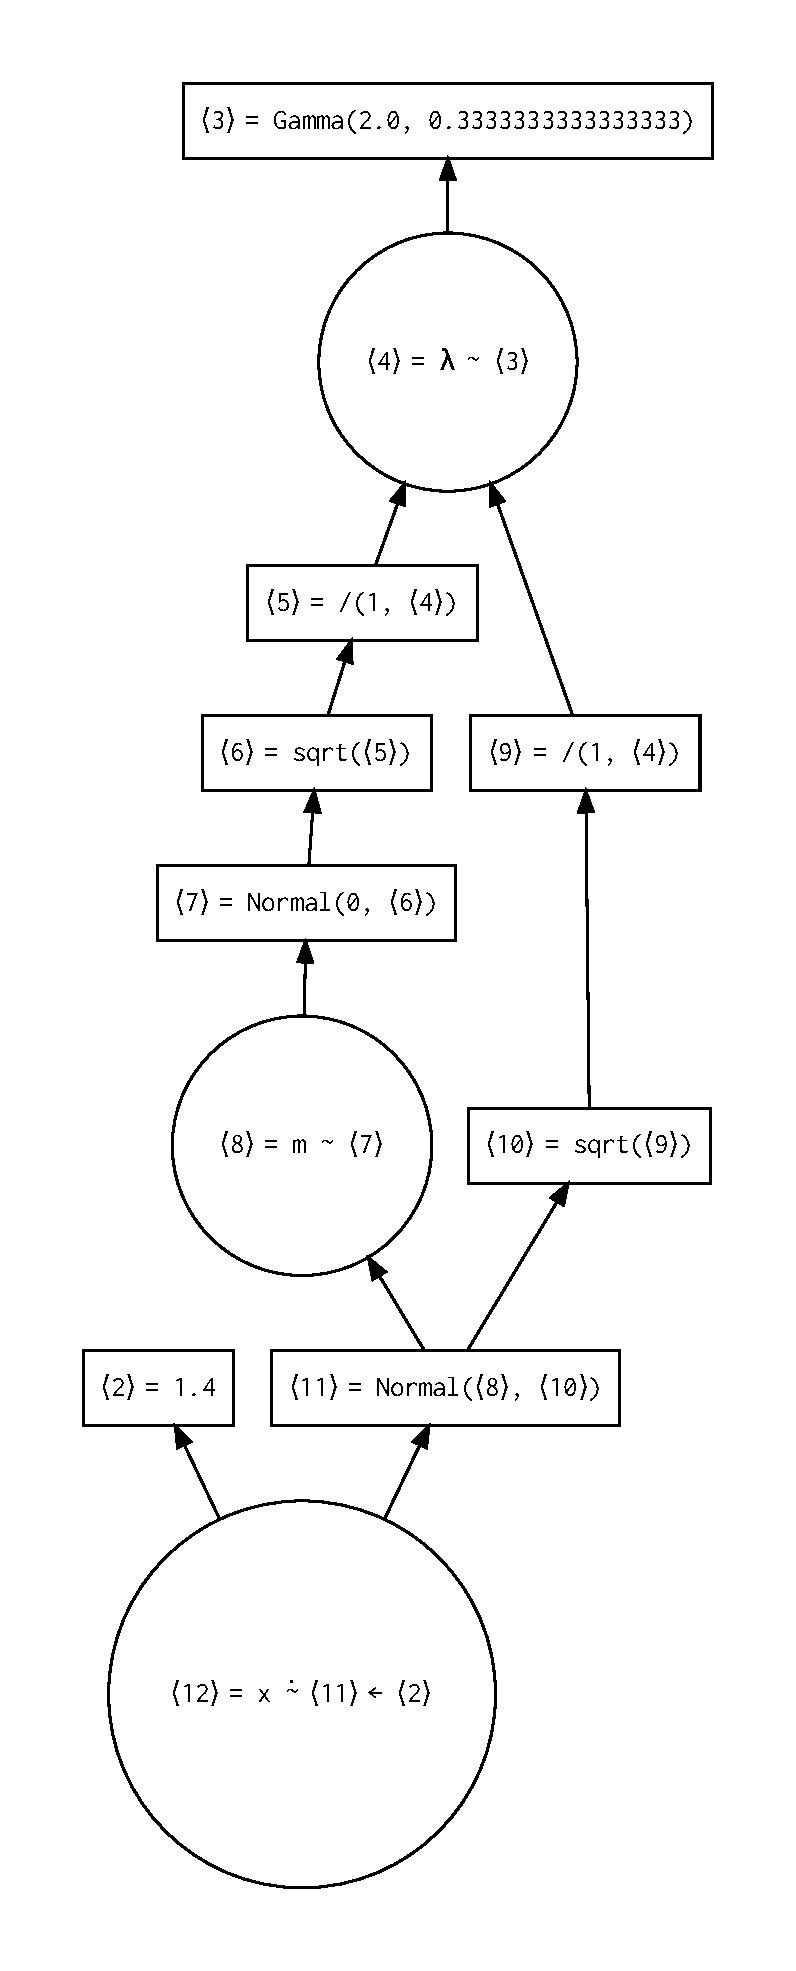
\includegraphics[width=0.49\textwidth]{figures/gaussian_dependencies}}
  \caption{Dependency graphs of the models in listing~\ref{lst:dependency-examples}, generated by
    \autogibbsjl{} and rendered by GraphViz.  More information, such as node values, is stored in
    the real model graph, but not printed for better readability.  Circular nodes denote tilde
    statements, while deterministic intermediate values, corresponding to normal SSA statements, are
    written in rectangles.}
  \label{fig:geom-deps}
\end{figure}


\section{Automatic Calculation of Gibbs Conditionals}
\label{sec:automatic-conditionals}

The ultimate contribution of this work is to utilize the dependency extraction system to extend
\turingjl{} with JAGS-style automatic calculation of Gibbs conditionals.  In JAGS (and its sibling,
BUGS) conditional extraction works over a wide range of variable types \parencite{plummer2003jags}
by symbolic analysis and recognition of several patterns, e.g., conjugate distributions from
exponential families, log-concave or compactly supported distributions; see
\textcite{lunn2000winbugs}.  This is possible since the class of models is constrained by the
modeling language, and available in completely structured form.

In \turingjl{}, models are much less restricted, and the symbolic form has to be recovered from
outside, as we have seen.  To focus on the principal ideas and not to extend the scope too much, the
implementation described in this section was restricted to the simpler case of finite, discrete
conditionals.  But since the construction of unnormalized conditionals densities, a necessary
intermediate step, is independent from the problem of normalization, this part could still serve as
a starting point for further, more general conditional samplers, as those in JAGS and BUGS.
Additionally, and this is a more fundamental limitation, the models to which the extraction
algorithm can be applied must be static in a specific sense: the whole Markov blanket of the
variable in question must be constant, unique, and reachable within one run of model tracking.  A
large fraction of the models used in practice do fulfill this condition, however, as counterexamples
would require stochastic control flow or non-constant supports.  As this problem is difficult to
solve in general, the same constraint applies to JAGS and BUGS, which makes \autogibbsjl{} not more
limited than these.

The implementation of the conditional extraction system involves three main steps:
\begin{enumerate}
  \firmlist
\item Extracting the symbolic form of the conditional likelihood of Markov blankets in a given
  dependency graph.
\item Constructing closures calculating the normalized discrete conditionals from these likelihoods.
\item Providing a Gibbs-component sampler for \turingjl{}, that can utilize the resulting
  conditional distributions.
\end{enumerate}
Alternatively, it would be possible to repeatedly trace the dependency graph and recalculate the
conditional likelihood at each Gibbs-component sampling step.  This could remediate some
restrictions, but at higher run-time cost.

The third of these steps turned out to be the easiest, since the sampling system of \turingjl{} is
designed to be extensible.  Ideally, a Gibbs-conditional sampler would have first been added to
\turingjl{} and then simply been reused for \autogibbsjl{}; in practice, it worked out the other way
round, and the \autogibbsjl{} sampler has, in generalized form, been added to \turingjl{} afterwards
(without the automatic extraction, only supporting user-provided conditional distributions).

\newsavebox{\bmlikelihoods}
\begin{lrbox}{\bmlikelihoods}
\begin{lstlisting}[style=lstfloat]
⟨2⟩ = false                 ⤳ false
⟨3⟩ = Dirichlet(2, 0.5)    ⤳ Dirichlet(2, 0.5)
⟨4⟩ = w ~ ⟨3⟩              ⤳ logpdf(Dirichlet(2, 0.5), θ[w])
⟨5⟩ = DNP([0.3, 0.7], ⟨4⟩) ⤳ DiscreteNonParametric([0.3, 0.7], θ[w])
⟨6⟩ = π ~ ⟨5⟩              ⤳ logpdf(DiscreteNonParametric([0.3, 0.7], θ[w]), θ[π])
⟨7⟩ = Bernoulli(⟨6⟩)       ⤳ Bernoulli(θ[π])
⟨8⟩ = x ~ ⟨7⟩ ← ⟨2⟩       ⤳ logpdf(Bernoulli(θ[π]), θ[x])
\end{lstlisting}
\end{lrbox}
\newsavebox{\hglikelihoods}
\begin{lrbox}{\hglikelihoods}
\begin{lstlisting}[style=lstfloat]
⟨2⟩ = 1.4                 ⤳ 1.4
⟨3⟩ = Gamma(2.0, 1/3)     ⤳ Gamma(2.0, 1/3)
⟨4⟩ = λ ~ ⟨3⟩             ⤳ logpdf(Gamma(2.0, 1/3), θ[λ])
⟨5⟩ = /(1, ⟨4⟩)           ⤳ /(1, θ[λ])
⟨6⟩ = sqrt(⟨5⟩)           ⤳ sqrt(/(1, θ[λ]))
⟨7⟩ = Normal(0, ⟨6⟩)      ⤳ Normal(0, sqrt(/(1, θ[λ])))
⟨8⟩ = m ~ ⟨7⟩             ⤳ logpdf(Normal(0, sqrt(/(1, θ[λ]))), θ[m])
⟨9⟩ = /(1, ⟨4⟩)           ⤳ /(1, θ[λ])
⟨10⟩ = sqrt(⟨9⟩)          ⤳ sqrt(/(1, θ[λ]))
⟨11⟩ = Normal(⟨8⟩, ⟨10⟩)  ⤳ Normal(θ[m], sqrt(/(1, θ[λ])))
⟨12⟩ = x ~ ⟨11⟩ ← ⟨2⟩    ⤳ logpdf(Normal(θ[m], sqrt(/(1, θ[λ]))), θ[x])
\end{lstlisting}
\end{lrbox}
\begin{figure}[t]
  \loosesubcaptions
  \subbottom[\texttt{bernoulli\_mixture(false)}]{\usebox{\bmlikelihoods}}
  \subbottom[\texttt{hierarchical\_gaussian(1.4)}]{\usebox{\hglikelihoods}}
  \caption{Association of the dependency graph of the example models from
    listing~\ref{lst:dependency-examples} with intermediate symbolic functions.  The expressions on
    the right are implicit functions of \protect\jlinl{θ}.  (\texttt{DNP} is used instead of
    \texttt{DiscreteNonParametric} to avoid breaking lines.)}
  \label{fig:continuations}
\end{figure}

The initial step, the symbolic extraction of likelihood functions, is implemented by first
converting the full trace into a symbolic joint log-density.  The expression of each node in the
dependency graph is therefore associated with a corresponding symbolic representation of a function
of the \enquote{trace dictionary} \jlinl{θ}, containing all values of the random variables by name
(which is to view the probabilistic model as a joint density over trace dictionaries).  This is done
in the following simple fashion:
\begin{itemize}
  \firmlist
\item References to call nodes or constant nodes (\jlinl{⟨i⟩ = x}) are inlined.
\item References to tilde nodes (\jlinl{⟨j⟩ = v ~ D}) are converted to dictionary lookups: \jlinl{θ[v]}.
\item Call nodes are converted to functions from the trace dictionary to a
  function call on the converted references: \jlinl{f(⟨i⟩, ⟨j⟩)} \(\leadsto\) \jlinl{f(x, θ[v])}.
\item Tilde nodes are converted to log-density evaluations of their values given the corresponding
  distribution: \jlinl{⟨j⟩ = v ~ D} \(\leadsto\) \jlinl{logpdf(D, θ[v])}
\end{itemize}
All resulting expressions are thereby to be understood as implicit functions of \jlinl{θ}.  These
new expression function objects can then be numerically evaluated as log-densities for given values
of all random variables.  For illustration, the joint densities of the \jlinl{bernoulli_mixture} and
\jlinl{hierarchical_gaussian} models introduced above in listing~\ref{lst:dependency-examples}, are
associated with corresponding symbolic functions as shown in figure~\ref{fig:continuations}\todo{fix
  caption alignment}.  By adding the log-likelihoods for each tilde statement, we get the symbolic
log-joint density as, for example,
\begin{lstlisting}
logpdf(Gamma(2.0, 0.33), θ[λ]) + 
  logpdf(Normal(0, sqrt(/(1, θ[λ]))), θ[m]) + 
  logpdf(Normal(θ[m], sqrt(/(1, θ[λ]))), θ[x]),
\end{lstlisting}
corresponding to the density over \(\lambda\), \(m\), and \(x\), factorized as
\begin{equation}
  p(\lambda, m, x) = p(\lambda) \, p(m \given \lambda) \, p(x \given m, \lambda).
\end{equation}
From this we can then derive conditionals by normalizing the proportional conditional, which can be
obtained by removing all terms of the joint factorization that do not depend on the conditioned
variable (cf. section~\ref{sec:bayes-infer}):
\begin{equation}
  \begin{aligned}
    p(m \given \lambda, x) &\propto p(m \given \lambda) \, p(x \given m, \lambda), \\
    p(\lambda \given m, x) &\propto p(\lambda) \, p(m \given \lambda) \, p(x \given m, \lambda),
  \end{aligned}
\end{equation}
which in more technical terms are given through the \emph{Markov blanket} of \(m\) and \(\lambda\)
\parencites[section 24.2]{murphy2012machine}[section 4.5]{koller2009probabilistic}.

The crucial problem here is to find the normalization factor.  In our case, within the constraint of
discrete and finite random variables, the normalization factor can be obtained exactly, as it
reduces to a finite sum.  (In the more general case, it could be found by analysing the structure of
the resulting expression, such as the conjugate variables \(m\), \(\lambda\), and \(x\) above, but
this is out of scope of the present work.)  For example, \(\pi\) in the \jlinl{bernoulli_mixture}
model is such a finitely supported variable~-- we get
\begin{equation}
    p(\pi \given w, x) = \frac{p(w) \, p(\pi \given w) \, p(x \given \pi)}{
      \sum_{\varpi \in \{0.3, 0.7\}}p(w) \, p(\varpi \given w) \, p(x \given \varpi)}.
\end{equation}
Since the distribution of every variable is preserved in the dependency graph, we can perform the
same operation programmatically, and turn the symbolic log-density into a distribution object by
simply tabulating the values of the denominator through evaluating of the expression over the whole
support of \(\pi\), the set \(\{0.3, 0.7\}\), and summing it up to get the normalization
factor.\footnote{This uses the interface of distribution objects from the
  \juliapackage{Distributions.jl} package, which have a \texttt{support} method whose result is an
  iterable object.}  This step finalizes the second of the three points of the scheme listed above.

To give a concrete illustration of the construction in programmatic terms, consider the
\jlinl{bernoulli_mixture} example:
\begin{enumerate}
  \firmlist
\item Find the likelihood expressions that match a given conditioned variable (this includes indexed
  variables subsumed by a parent, like \jlinl{v[i]} and \jlinl{v}), and their distribution:
  \begin{equation*}
    \begin{aligned}
      \ell_{1} &= \mathtt{logpdf(DiscreteNonParametric([0.3, 0.7],\theta[w]), \theta[\pi])}. \\
      \mathcal{D} &= \mathtt{DiscreteNonParametric([0.3, 0.7], \theta[w])}.
    \end{aligned}
  \end{equation*}
\item For each of these (sub-)variables, collect the likelihoods of their children variables, thus
  completing the Markov blanket:
  \begin{equation*}
    \ell_{2} = \mathtt{logpdf(Bernoulli(\theta[\pi]), \theta[x])}.
  \end{equation*}
  The complicated part of this and the previous step is the correct matching of indexed variables in
  the trace dictionary: forms like \jlinl{θ[v][1]} and \jlinl{θ[v[1]]} need to be resolved correctly
  to the same value.
\item Construct for each conditioned variable a closure function that takes as an argument a fixed
  trace dictionary, tabulates the conditional log-likelihood over it with the conditioned variable
  fixed to all values of its support, and normalizes the result: let
  \begin{equation*}
    \Omega = \mathtt{support}(\mathcal{D}) = \mathtt{[0.3, 0.7]},
  \end{equation*}
  then the closure is
  \begin{equation*}
    \theta \mapsto \distr{DiscreteNonParametric}(\Omega, \operatorname{softmax}(\mathtt{table}(\theta)))
  \end{equation*}
  where
  \begin{equation*}
    \mathtt{table}(\theta)_i = \operatorname{eval}(\ell_{1}, \theta[\pi \leadsto \Omega_i]) +
    \operatorname{eval}(\ell_{2}, \theta[\pi \leadsto \Omega_i])
  \end{equation*}
  are the unnormalized log-likelihoods.
  % \begin{equation*}
  %   \begin{aligned}
  %     &\theta \mapsto \{ \\
  %     &\quad \mathtt{table} = \left[\operatorname{eval}(\ell_{1}, \theta[\pi \leadsto \varpi]) +
  %       \operatorname{eval}(\ell_{2}, \theta[\pi \leadsto \varpi]) \mid \varpi \in \Omega \right] \\
  %     &\quad \distr{DiscreteNonParametric}(\Omega, \operatorname{softmax}(\mathtt{table})) \\
  %     &\}.
  %   \end{aligned}
  % \end{equation*}
  Here, \(\operatorname{softmax}(x) = \broadcast{\exp}(x) / \sum_i \exp(x_{i})\) is the
  normalization operation on log-probabilities, \(\mathrm{eval}\) the evaluation function for
  likelihood closures, and \(\theta[v \leadsto x]\) denotes setting the value of variable \(v\) in
  \(\theta\) to~\(x\).\todo{orphan}
\end{enumerate}
The result of this process is a collection of closures that represent the conditional likelihoods as
\enquote{kernels}: functions from conditioned-on variables to distribution objects.  These closures
can then be used to construct a conditional sampler for usage in \turingjl{}'s \jlinl{Gibbs}
sampler, in combination with other samplers for the continuous variables.

\newthought{As for potential improvements}, there is of course a wide range of possibilities for
extension.  As mentioned before, further classes of random variables beyond those with finite
support could be handled, using methods and heuristics as in BUGS or JAGS.  This could also involve
symbolic methods such as in AutoConj \parencite{hoffman2018autoconj}. More generally,
variance-reducing transformations, e.g., the Rao-Blackwellization from \textcite{murray2017delayed},
are applicable.  Furthermore, as done in \juliapackage{Gen.jl}, a variant of \enquote{argument
  diffs} could be devised to prevent unnecessary re-evaluation of model parts
\parencites[see][section 1.2.3]{cusumano-towner2020gen}{becker2020dynamic} (a technique that could
also be used to improve efficiency of particle samplers).

Besides improvements via inference algorithms, it would be possible for models that are written in a
vectorized or otherwise \enquote{trace constant} fashion, such that the structure of the
conditionals does not change with the number of observations, to record the trace for a small model
and reuse it for arbitrary larger ones, thus avoiding recomputation and recompilation.  Finally, the
evaluation of the conditional closures, which is currently performed by simple interpretation of
expressions, could be sped up by compiling them to Julia methods, or even better by reusing the
SSA-like structure to emit Julia IR directly.

A more radical approach would be to move away from working on a trace-based reconstruction obtained
at run-time.  Such an idea, using a PPL-specific intermediate representation of the complete model
program, with generalized transformation capabilities, is outlined in section~\ref{sec:future-work}
below.  This could allow more invariance with respect to inference algorithms, and would enable
handling more general probabilistic models (foremost, not only static ones).


\section{Evaluation}
\label{sec:autogibbs-eval}

\autogibbsjl{} is a prototype.  There is still some slowness resulting from compilation, and therein
primarily type inference, of the functions handling all the strongly typed expression trees.
Besides the possibility of just optimizing these further, the following fact is most important to
realize: compilation takes place only once~-- as soon as a conditional is constructed, it can be
reused in arbitrarily many sampling runs of the same model.  The finished conditionals then do not
take so much time anymore, quite the contrary: they are much faster than other within-Gibbs
samplers, since they only involve evaluating a fixed expression, constructing a distribution, and
sampling from it once (and even this could be sped up further).  This makes it possible to sample
much longer chains in the same time, which is an overall advantage.

Furthermore, due to the limitations \autogibbsjl{} puts on the structure of variable names and
indexing, there are cases in which models cannot be formulated in a some specific way in \dppljl{},
thus losing certain advantages such as block-wise treatment of collections of independent variables.
Again, the restrictions are mostly a detail of the current implementation.  Based on the lessons
learned through this work, further improvements to Gibbs sampling in \turingjl{} are already
planned.

\newthought{Besides several unit tests} for correctness of the derived dependencies and conditionals
on a variety of small models chosen to test certain features and corner cases, an experimental
comparison of \autogibbsjl{} and existing \turingjl{} samplers has been conducted.  Three
off-the-shelf Bayesian models were chosen: a Gaussian mixture model (GMM) with \(N\) observations,
\(K\) clusters, known variances \(\sigma\), and priors over cluster centers \(\mu\), weights \(w\), and
assignments \(z\) \parencite[section 6.2]{marin2007bayesian}:
\begin{equation}
  \label{eq:gmm}
  \begin{aligned}
    w &\from \distr{Dirichlet(K)}, \\
    z_{n} &\from \distr{Categorical}([1, \ldots, K], w), \quad\text{for } 1 \le n \le N, \\
    \mu_{k} &\from \Normal(0, \sigma_{1}), \quad\text{for } 1 \le k \le K, \\
    x_{n} &\from \Normal(\mu_{z_{n}}, \sigma_{2}), \quad\text{for } 1 \le n \le N;
  \end{aligned}
\end{equation}
a hidden Markov model (HMM) with \(N\) observations, \(K\) clusters, known variances \(\sigma\), and
priors over transition (\(T\)) and emission (\(m\)) probabilities \parencite[section
7.3]{marin2007bayesian}:
\begin{equation}
  \label{eq:hmm}
  \begin{aligned}
    T_{k} &\from \distr{Dirichlet}(K), \quad\text{for } 1 \le k \le K, \\
    m_{k} &\from \Normal(k, \sigma_{1}), \quad\text{for } 1 \le k \le K, \\
    s_{1} &\from \distr{Categorical}([1, \ldots, K], [1/K, \ldots, 1/K]), \\
    s_{n} &\from \distr{Categorical}([1, \ldots, K], T_{s_{n-1}}), \quad\text{for } 2 \le n \le N, \\
    x_{n} &\from \Normal(m_{s_{n}}, \sigma_{2}), \quad\text{for } 1 \le n \le N;
  \end{aligned}
\end{equation}
and a \(K\)-truncated infinite mixture model (IMM) with \(N\) observations, in stick-breaking
construction with fixed parameter \(\alpha\), but otherwise of the same form as the GMM, to
represent a nonparametric example \parencite[section 2.2]{hjort2010bayesian}:
\begin{equation}
  \label{eq:imm}
  \begin{aligned}
    w &\from \distr{TruncatedStickBreakingProcess(\alpha, K)}, \\
    z_{n} &\from \distr{Categorical}([1, \ldots, K], w), \quad\text{for } 1 \le n \le N, \\
    \mu_{k} &\from \Normal(0, \sigma_{1}), \quad\text{for } 1 \le k \le K, \\
    y_{n} &\from \Normal(\mu_{z_{n}}, \sigma_{2}), \quad\text{for } 1 \le n \le N.
  \end{aligned}
\end{equation}
The concrete values of all involved hyper-parameters can be found in the test directory of the
published source
code\footnote{\protect\href{https://github.com/phipsgabler/AutoGibbs.jl/tree/2b433f8f5c37a55f63fbf175193130b46c8b569f/test}{https://github.com/phipsgabler/AutoGibbs.jl/tree/master/test}}.

The three interesting classes of metrics in the context of this work are:
\begin{enumerate}
  \firmlist
\item the \enquote{extraction time} of \autogibbsjl{}, i.e., the time it takes to extract and a
  conditional including compilation times,
\item the sampling speed when used as component of a within-Gibbs sampler, and
\item the quality of the resulting chains, in terms of convergence and variance diagnostics.  (Note
  that while this really benchmarks Gibbs sampling, not the implementation of \autogibbsjl{}, it is
  a relevant comparison for the practitioner.)
\end{enumerate}
These quantities were estimated on each of the test models, which all involve one discrete and two
continuous parameter arrays.  As a baseline for \autogibbsjl{}'s static conditional (AG),
\turingjl{}'s Particle Gibbs sampler (PG; \textcite[see]{andrieu2010particlea}) was chosen, which is
also suited to discrete parameters.  PG was always used with \(100\) particles, since lower values
did not lead to convergent chains.  Continuous variables were sampled using Hamiltonian Monte Carlo
(HMC; \textcite[see]{betancourt2018conceptual}) with hand-tuned parameters (\(10\) leapfrog steps
with step size \(0.05\)).  The experiments have been set up to vary between AG and PG, and between
\(10\), \(25\), and \(50\) observations, since this number determines the size of the trace, and
thus influences both AG's compile times and the overall sampling time.  All measurements were
conducted using the following system configuration, as shown by
\jlinl{InteractiveUtils.versioninfo()}:\todo{page break?}
\begin{lstlisting}
Julia Version 1.3.1
Commit 2d5741174c (2019-12-30 21:36 UTC)
Platform Info:
  OS: Linux (x86_64-pc-linux-gnu)
  CPU: Intel(R) Core(TM) i5-4690 CPU @ 3.50GHz
  WORD_SIZE: 64
  LIBM: libopenlibm
  LLVM: libLLVM-6.0.1 (ORCJIT, haswell)
\end{lstlisting}
Everything was executed single-threaded, with exclusive resource access on the server, to preclude
measurement noise as much as possible.  Each of the three models was benchmarked in a separate Julia
session, starting with a fixed random seed.  The last two chains of the HMM with \(50\) observations
using Particle Gibbs could not be completed, due to the twelve hour time limit set by the job
scheduler.  The raw data can be found online in
\textcite{gabler2020mcmc}\footnote{\protect\url{https://doi.org/10.5281/zenodo.4307916}}.

The \dppljl{} implementations of the models can be found in listing~\ref{lst:evaluation-models}.
Note that for each, there exists a second, equivalent implementation used for PG, since particle
samplers in \turingjl{} require the usage of special data types due to their task copying mechanism.

\newthought{It follows} a detailed analysis of the results per model in graphical form, based on six
plots each.  First, PG and AG are compared in terms of sampling times by number of observations on
the top left.  Right of this, we have the dependency of the extraction time of AG given the number
observations.  The first of these points is almost always an outlier, since it involves additional
compilation time.  Through the rest, a quadratic function is fitted, which always matched the values
very closely.

On the recto pages, plots for convergence analysis are visualized.  Since these are estimated per
parameter, and the test models involve larger arrays of parameters, the first elements of the
continuous and the fifth element of the discrete parameters have always been chosen as
representatives.  On the top, the first chain of each experimental combination is shown as a
qualitative representative (thinned for ease of plotting).  Well-converging chains should look like
stationary processes~-- more like white noise than a random walk.  In the middle plot, the estimated
autocorrelation functions of the same chains are given, which are a way to evaluate convergence
speed by eye.  The functions should vanish quickly (indicated by the gray significance bar around
the abscissa); perfectly uncorrelated chains would have vanishing autocorrelation except for lag
zero.

Lastly, two diagnostic values are plotted for each combination and chain.  The
\enquote{scale-reduction} \(\widehat{\mathrm{R}}\), after \textcite{gelman1992inference}, estimates
the factor by which the scale of the current distribution might be reduced if the simulations were
continued \parencite[see][p. 285]{gelman2020bayesian}.  It should be close to one for indicating
good convergence; as a rule of thumb, a value of more than \(1.1\) is suspicious.  The effective
sample size (ESS) arises in the estimation of the asymptotic variance of Markov chains
\parencite[][section 7.2]{vihola2020lectures}, where it is formally analogous to the sample size in
the central limit theorem for \iid{} variables.  The ESS can also be interpreted as a one-point
summary of the autocorrelation estimate, normalized by chain length.  It should be close to the
actual number of samples, or at least of the same order of magnitude.

%%%%%%%%%%%%%%%%%%%%%%%%%%%%%%%%%%%%%%%%%%%%%%%%%%%%%%%%%%%%%%%%%%

\begin{lstfloat}[p]
\begin{lstlisting}[style=lstfloat]
@model function gmm(x, K)
    N = length(x)
    w ~ Dirichlet(K, 1/K)  # Cluster association prior
    z ~ filldist(Categorical(w), N)  # Cluster assignments
    μ ~ filldist(Normal(0.0, s1_gmm), K)  # Cluster centers

    for n = 1:N
        x[n] ~ Normal(μ[z[n]], s2_gmm)  # Observations
    end
end

@model function hmm(x, K, ::Type{T}=Float64) where {T<:Real}
    N = length(x)

    T = Vector{Vector{X}}(undef, K)
    for i = 1:K
        T[i] ~ Dirichlet(K, 1/K)  # Transition probabilities
    end
    
    s = zeros(Int, N)
    s[1] ~ Categorical(K)
    for i = 2:N
        s[i] ~ Categorical(T[s[i-1]])  # State sequence
    end
    
    m = Vector{T}(undef, K)
    for i = 1:K
        m[i] ~ Normal(i, s1_hmm)  # Emission probabilities
    end
    
    x[1] ~ Normal(m[s[1]], s2_hmm)
    for i = 2:N
        x[i] ~ Normal(m[s[i]], s2_hmm)  # Observations
    end
end

@model function imm_stick(y, α, K)
    N = length(y)
    crm = DirichletProcess(α)
    v ~ filldist(StickBreakingProcess(crm), K - 1)
    w = stickbreak(v)  # Cluster weights
    
    z = zeros(Int, N)
    for n = 1:N
        z[n] ~ Categorical(w)  # Cluster assignments
    end

    μ ~ filldist(Normal(0.0, s1_imm), K)  # Cluster centers

    for n = 1:N
        y[n] ~ Normal(μ[z[n]], s2_imm)  # Observations
    end
end
\end{lstlisting}
  \caption{Gaussian mixture model, hidden Markov model, and infinite mixture model using a
    stick-breaking construction.  The two-step calculation of \texttt{w} via \texttt{v} is a
    technicality due to \turingjl{}'s handling of nonparametric models.  The function
    \texttt{stickbreak} normalizes the stick-lengths \texttt{v} into a Dirichlet-like distribution.
    The \texttt{Categorical(p)} constructor automatically infers the support of the categorical
    distribution from the weight vector as \texttt{1:length(p)}.}
  \label{lst:evaluation-models}
\end{lstfloat}

%%%%%%%%%%%%%%%%%%%%%%%%%%%%%%%%%%%%%%%%%%%%%%%%%%%%%%%%%%%%%%%%%%
\cleartoverso
\FloatBlock

\newcommand{\leftplotcaption}[1]{%
  Sampling and extraction times for #1, factored by algorithm and number of observations.  Points
  are jittered horizontally to increase readability.  A quadratic curve is fitted to the extraction
  times.
}

\newcommand{\rightplotcaption}[1]{%
  Diagnostics, factored by algorithm, number of observations, and a selection of model parameters.
  \(\widehat{\mathrm{R}}\) and ESS point estimates are jittered horizontally for better readability.
  A horizontal line marks the reference value of \(1.1\) in the \(\widehat{\mathrm{R}}\) plot.  For
  chain plots and autocorrelation, the third chain of the respective combination has been used.
}

\begin{figure}[t!]
  \centering
  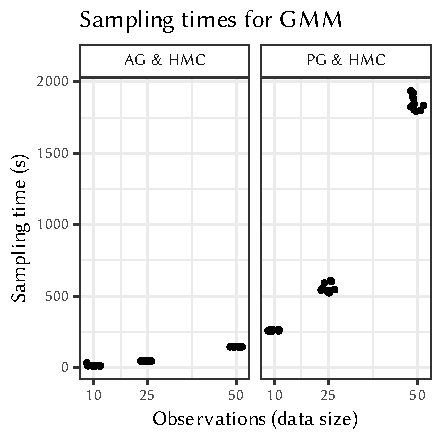
\includegraphics[width=0.49\textwidth]{figures/GMM-sampling_times}
  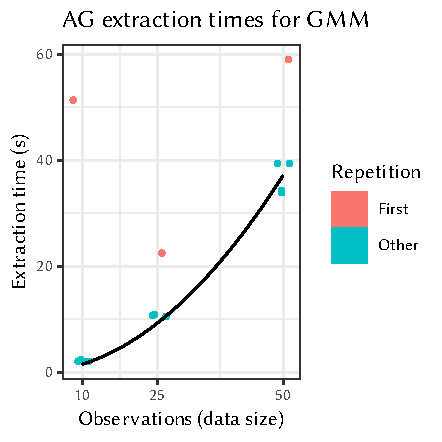
\includegraphics[width=0.49\textwidth]{figures/GMM-compile_times}
  \caption{\leftplotcaption{GMM}}
  \label{fig:plots-gmm-left}
\end{figure}

\subsection*{Gaussian Mixture Model}

For the GMM, the AG sampling times (figure~\ref{fig:plots-gmm-left}, left) lie consistently below the
minimum of the PG sampling times, even with the largest number of observations.  Extraction time
(on the right) seems to grow quadratically, with exception of the first call of
the conditional extraction, involving compilation and type inference.

The mixing behavior of the chains (figure~\ref{fig:plots-gmm-right}, top) shows a large variation.
With \(10\) and \(25\) observations, neither of the algorithms reaches consistently satisfactory
results; the distribution of \(\widehat{R}\) values (bottom left) is quite diffuse and suspiciously
large (more so for PG), and especially the ESS (bottom right) is way too low.  A look at the
exemplary autocorrelation plots (middle) seems to confirm bad convergence.  The corresponding chains
clearly show random-walk-like or \enquote{lumped} behavior for some combinations.

For \(50\) observations, the result is different with AG.  The \(w\) and \(\mu\) parameters appear
to converge well in most cases, with very low-variance chains and visibly large ESS values.  But for
unknown reasons, the \(z\) parameter seems to have gotten \enquote{stuck} in this particular example
and not moved at all, which is the reason no autocorrelation function could be estimated.  PG might
have improved somewhat, looking at the lower \(\widehat{R}\) distributions, but not enough to make a
meaningful difference, as ESS and autocorrelation plots show no sufficiently good behavior.


\cleartorecto
\FloatBlock

\begin{figure}[p]
  \centering
  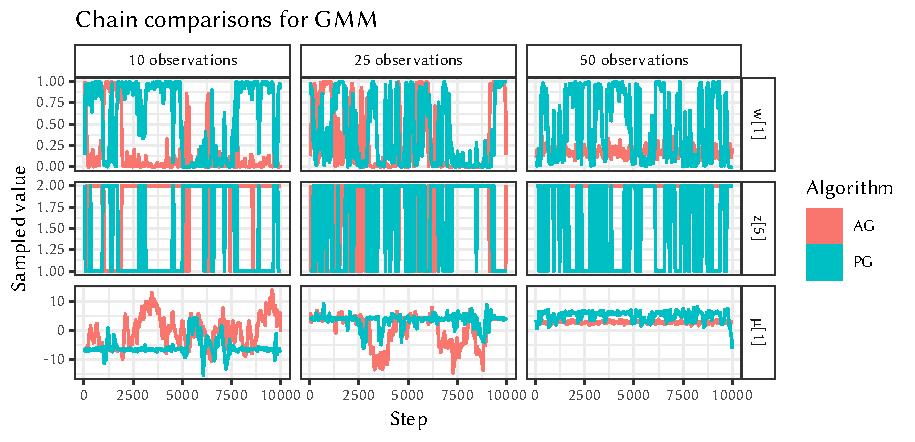
\includegraphics[width=\textwidth]{figures/GMM-chains}
  \par
  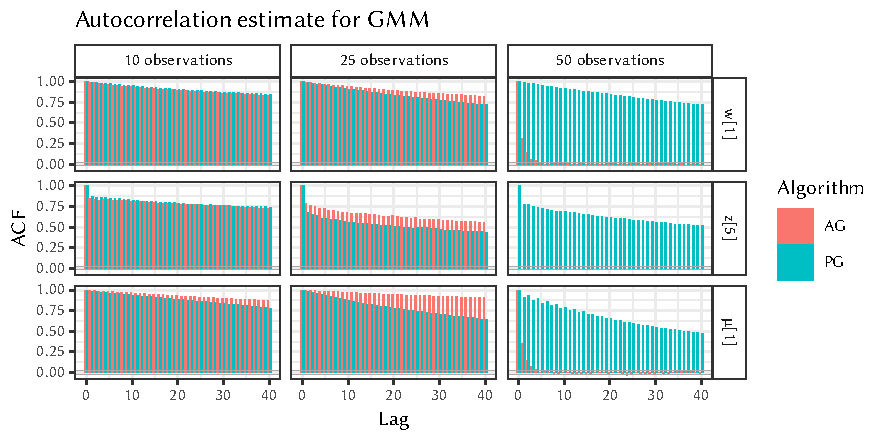
\includegraphics[width=\textwidth]{figures/GMM-acfs}
  \par
  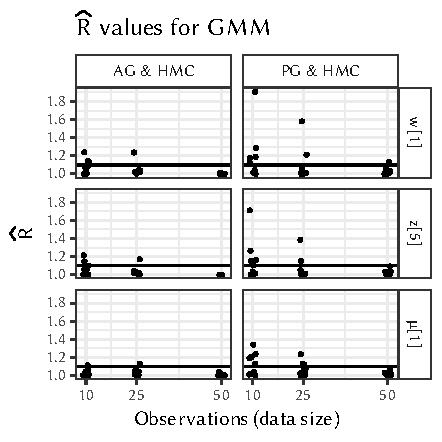
\includegraphics[width=0.49\textwidth]{figures/GMM-rhat}
  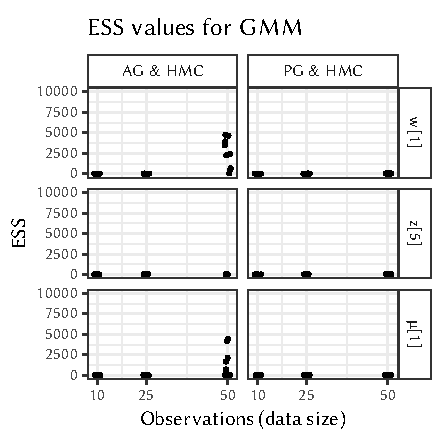
\includegraphics[width=0.49\textwidth]{figures/GMM-ess}
  \caption{\rightplotcaption{GMM}}
  \label{fig:plots-gmm-right}
\end{figure}

%%%%%%%%%%%%%%%%%%%%%%%%%%%%%%%%%%%%%%%%%%%%%%%%%%%%%%%%%%%%%%%%%%
\cleartoverso
\FloatBlock

\begin{figure}[t!]
  \centering
    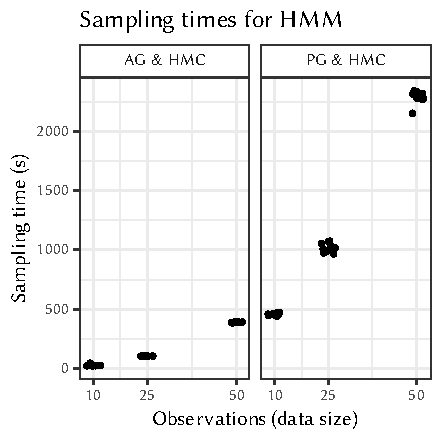
\includegraphics[width=0.49\textwidth]{figures/HMM-sampling_times}
  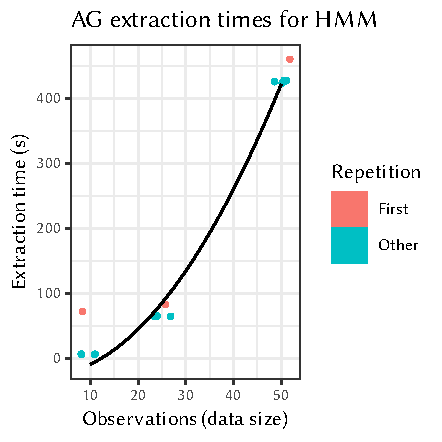
\includegraphics[width=0.49\textwidth]{figures/HMM-compile_times}
  \caption{\leftplotcaption{HMM}}
  \label{fig:plots-hmm-left}
\end{figure}

\subsection*{Hidden Markov Model}

Also for HMM, the same trends in sampling and extraction times as with GMM are visible
(figure~\ref{fig:plots-hmm-left}), with AG being consistently faster.  The extraction times seem to
be quite the same as GMM, even in absolute terms, as are the outliers of the first function calls.

Mixing behavior for this model is much better overall.  The chains
(figure~\ref{fig:plots-hmm-right}, top) look less like random walks, especially for \(\mu\).
Autocorrelation plots (middle) are sometimes quite good, especially for \(s\), and in all cases
better as those above for GMM.  The \(\widehat{R}\) values (bottom left) are all in better ranges
(note the difference in the scale of the ordinate!), and ESS (bottom right) noticeably higher.
Overall, AG seems to improve over PG on average, to some degree.

\cleartorecto
\FloatBlock

\begin{figure}[p]
  \centering
  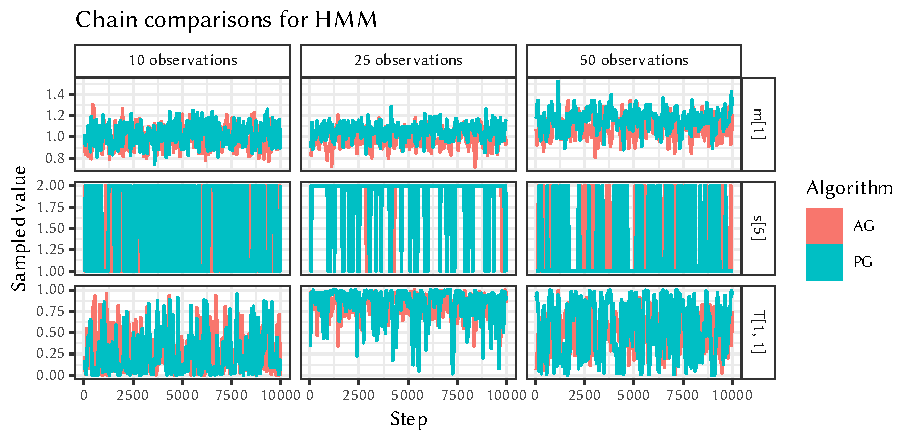
\includegraphics[width=\textwidth]{figures/HMM-chains}
  \par
  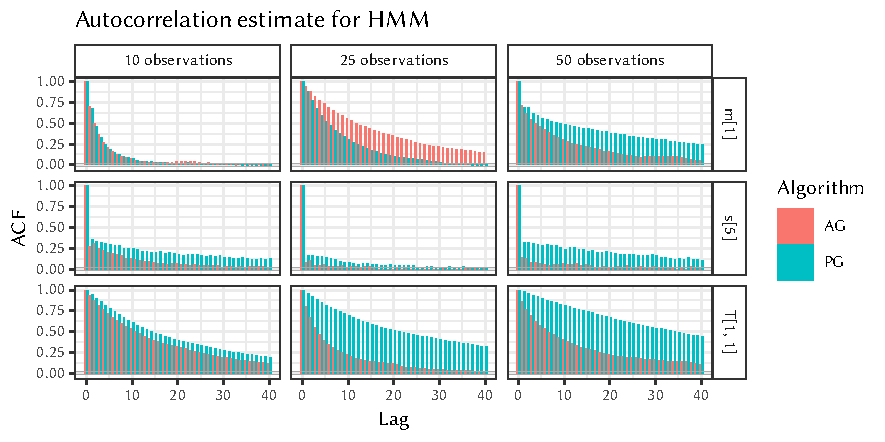
\includegraphics[width=\textwidth]{figures/HMM-acfs}
  \par
  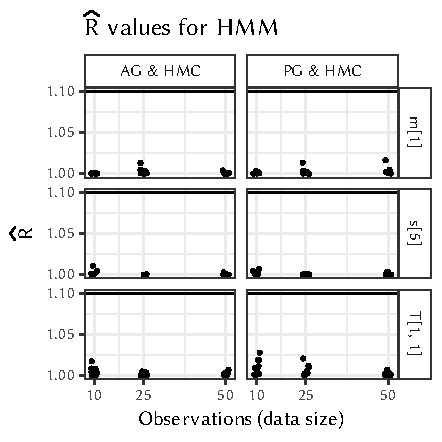
\includegraphics[width=0.49\textwidth]{figures/HMM-rhat}
  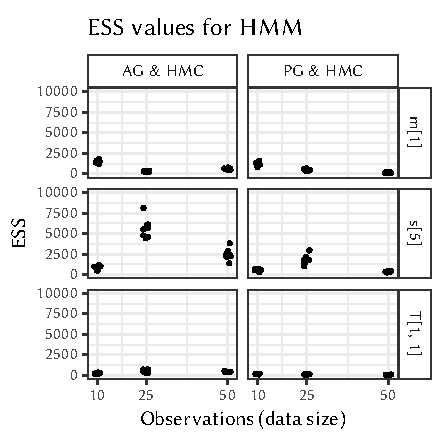
\includegraphics[width=0.49\textwidth]{figures/HMM-ess}
  \caption{\rightplotcaption{HMM}}
  \label{fig:plots-hmm-right}
\end{figure}

%%%%%%%%%%%%%%%%%%%%%%%%%%%%%%%%%%%%%%%%%%%%%%%%%%%%%%%%%%%%%%%%%%
\cleartoverso
\FloatBlock

\begin{figure}[t!]
  \centering
  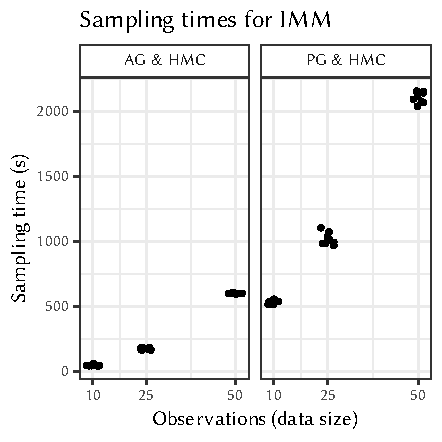
\includegraphics[width=0.49\textwidth]{figures/IMM-sampling_times}
  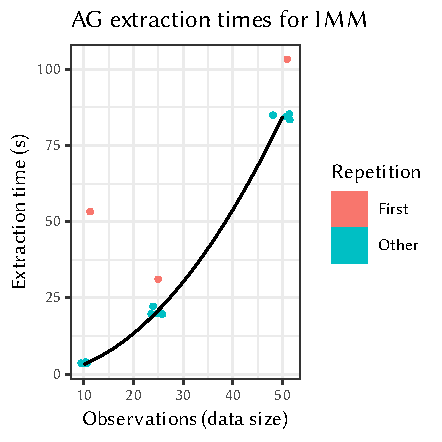
\includegraphics[width=0.49\textwidth]{figures/IMM-compile_times}
  \caption{\leftplotcaption{IMM}}
  \label{fig:plots-imm-left}
\end{figure}


\subsection*{Infinite Mixture Model}

Again, similar trends of sampling times and extraction times (figure~\ref{fig:plots-imm-left}) are
noticeable.  Here we can observe some larger involved factors, though; both curves grow faster, with
PG on \(10\) observations even being faster than AG on \(50\) observations; although still on a
significantly higher scale in general.

In this example, PG appears to work better on average.  In the example chain plots
(figure~\ref{fig:plots-imm-right}, top), we can only see a noticeable difference for \(\mu\), while the
autocorrelation graphs (middle) are almost all worse for AG (although both algorithms seem to do
better than in the GMM test).  ESS (bottom right) is only satisfactory for the \(z\) parameters, but
PG here shows a much more consistent behavior of the \(\widehat{R}\) distribution (bottom left).

\begin{figure}[p]
  \centering
  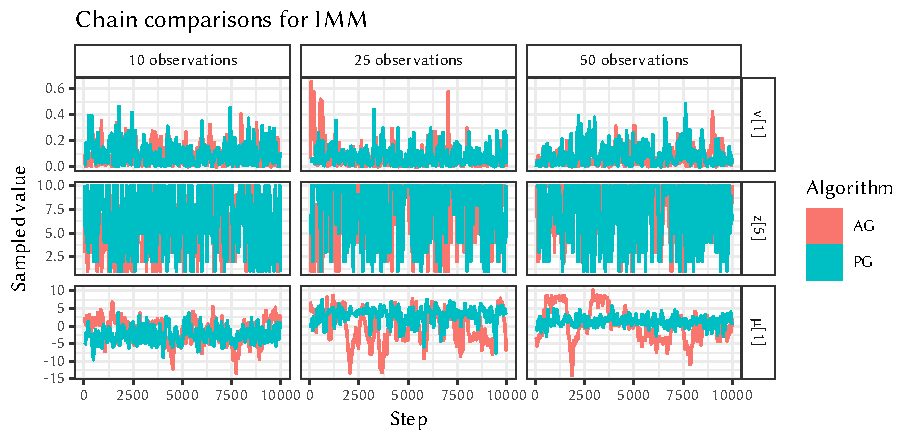
\includegraphics[width=\textwidth]{figures/IMM-chains}
  \par
  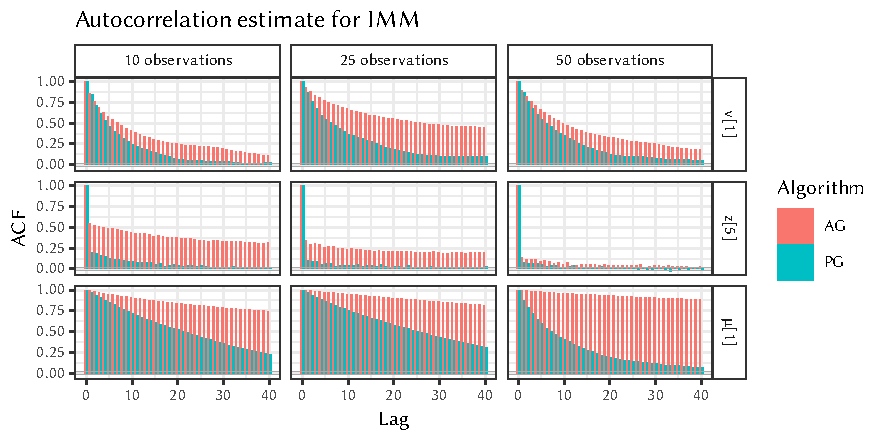
\includegraphics[width=\textwidth]{figures/IMM-acfs}
  \par
  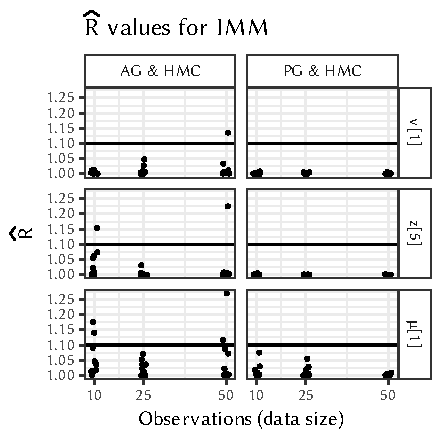
\includegraphics[width=0.49\textwidth]{figures/IMM-rhat}
  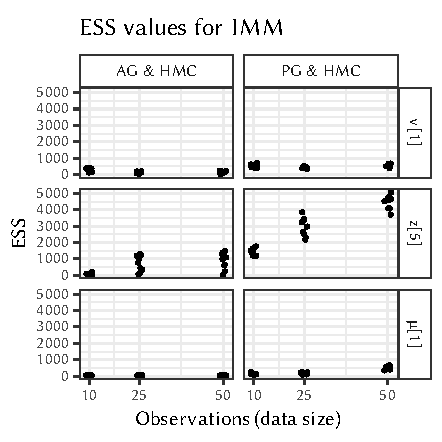
\includegraphics[width=0.49\textwidth]{figures/IMM-ess}
  \caption{\rightplotcaption{IMM}}
  \label{fig:plots-imm-right}
\end{figure}

\FloatBlock
\clearpage

\subsection*{Summary}

Whereas the sampling times of PG always grow rather fast, depending on the number of observations,
the rate of growth seems to be much lower for AG.  The behavior of these curves appears to be
superlinear, perhaps quadratic.  For GMM and HMM, the maximal sampling time of AG is always below
the minimal sampling time of PG.  Even in the case of IMM, AG's sampling time with \(50\)
observations is closest to PG's with only \(10\) particles, with the latter still obviously rising
much faster.

With regard to the extraction times, we can note a pretty clear quadratic run-time depending on the
number of observations.  The first run is always significantly above this trend, due to the impact
of compilation and type inference.  Additionally, the first invocation for the lowest number of
observations might have involved additional compilation of library functions, explaining the larger
residual compared to the first runs of the larger numbers.

In terms of convergence, AG and PG deliver quite comparable results, varying with some variation in
quality depending on model and number of observations.  In most cases, judging by eye through the
exemplary autocorrelation plots, one or the other seems to slightly beat the other, which is
buttressed by the distribution of the diagnostic values.  IMM seems poses a particularly bad
application for AG, but otherwise, no consistent \enquote{winner} is visible, and variations do not
seem to follow a consistent pattern.

In conclusion, it can be said that for models where both are applicable,
\juliapackage{Auto\-Gibbs.jl} provides a viable alternative to PG, delivering comparable results in
less time.  Care has to be taken to diagnose mixing behavior, though, as always in MCMC simulations.


% \begin{table}[t]
%   \centering
%   \libertineTabular
%   \begin{tabularx}{\textwidth}{XXrrr@{\hskip 10mm}rrrr}
%     \toprule
%      & & \multicolumn{3}{c@{\hskip 10mm}}{\textbf{GMM}} & \multicolumn{3}{c}{\textbf{HMM}} & \multicolumn{1}{c}{\textbf{IMM}} \\
%     \midrule
%     & HMC Step size & & 0.05 & & & 0.05 & & 0.05 \\
%     & HMC Steps & & 10 & & & 10 & & 10 \\
%     \midrule
%     \textbf{AG + HMC} & Observations & 10 & 25 & 50 & 10 & 25 & 50 & 10 \\
%     & Chains & 30 & 30 & 30 & 30 & 30 & 30 & 30 \\
%     & Compilations & 3 & 3 & 3 & 3 & 3 & 3 & 3 \\
%     \addlinespace
%     \textbf{PG + HMC,} & Observations & 10 & 25 & 50 & 10 & 25 & 50 & 10 \\
%      & Chains & 10 & 10 & 10 & 10 & 10 & 10 & 10 \\
%     \bottomrule
%   \end{tabularx}
%   \caption{Experimental conditions for evaluating AutoGibbs (AG) against Particle Gibbs (PG).  Chains
%     were always of length \(10000\).  A new static Gibbs conditional was extracted for each block of
%     \(10\) chains that was run with the same parameters while Particle Gibbs was varied over the
%     three particle sizes.  Particle Gibbs with 50 particles was sometimes killed due to timeouts on
%     the server.}
%   \label{tab:autogibbs-params}
% \end{table}



% extraction times
% Measuring both compilation of the traced code and the conditional calculation.",
% "All 2 or 3 repetitions per data size class are shown."
% Linear fit for time ~ datasize²
% three samples

% sampling times
% subtitle = "Factored by algorithm and number of PG particles"

% diagnostics
% subtitle = "Factored by algorithm and number of particles"

% densities
% subtitle = paste("Factored by number of observations (data size)", "and selected parameters")

% ACFs
% subtitle = "ACF plots for one sample chain per data size"


%%% Local Variables: 
%%% TeX-master: "main"
%%% End: